\section{Auswertung}
\label{sec:Auswertung}

\subsection{Verifizierung der Linsengleichung und des Abbildungsgesetzes}
\label{sec:brennweite1}

In Tab. \ref{tab1} sind die Gegenstandsweite $g$, die Brennweite $b$ und die Bildgröße $B$ aufgelistet. Die Gegenstandsgröße beträgt $G = \SI{3}{\centi\meter}$.

\begin{table}\caption{Der maximale Drehimpuls $L$, der Gesamtspin $S$ und der Gesamtdrehimpuls $J$ ergeben sich zum Landé-Faktor $g_\text{J}$ für die vier verschiedenen Elemente.}
\label{tab1}
\centering
\sisetup{round-mode = places, round-precision=2, round-integer-to-decimal=true}
\begin{tabular}{S[]S[]S[]S[]} 
\toprule
{$L$} & {$S$} & {$J$} & {$g_\text{J}$}\\
\midrule
5.0 & 1.0 & 4.0 & 0.8\\
0.0 & 3.5 & 3.5 & 2.0\\
6.0 & 1.5 & 4.5 & 0.7272727272727273\\
5.0 & 2.5 & 7.5 & 1.3333333333333333\\
\bottomrule
\end{tabular}\end{table}

\noindent Aus den Werten für die Bildweite $b$ und die Gegenstandsweite $g$ ergibt sich mit Gleichung {eqn:abbildungsgesetz} der Mittelwert des Abbildungsmaßstabes $V$ zu 
\begin{equation*}
    V_\text{Var1} = \num{1.5 \pm 0.7}.
\end{equation*}

\noindent Aus den Werten für die Bildgröße $B$ und die Gegenstandsgröße $G$ ergibt sich mit Gleichung \eqref{eqn:abbildungsgesetz} der Mittelwert des Abbildungsmaßstabes $V$ zu
\begin{equation*}
    V_\text{Var2} = \num{1.4 \pm 0.6}.
\end{equation*}

\noindent Nach Gleichung \eqref{eqn:linsengleichung} ergibt sich für die Brennweite $f$ ein Wert von 
\begin{equation*}
    f = \SI{9.62 \pm 0.05}{\centi\meter}.
\end{equation*}

\noindent Die Herstellerangabe gibt für die Brennweite einen Wert von 
\begin{equation*}
    f_\text{real} = \SI{10}{\centi\meter}
\end{equation*}
an.

\noindent Um die Messgenauigkeit visuell erkennen zu können, werden die Werte $b$ und $g$ als Schnittpunkte mit der $x$- und $y$-Achse betrachtet. Die zueinandergehörenden Werte werden verbunden und es wird geschaut, in welchem Punkt sich die Geraden schneiden (Abb. \ref{brennweite}).

\begin{figure}
    \centering
    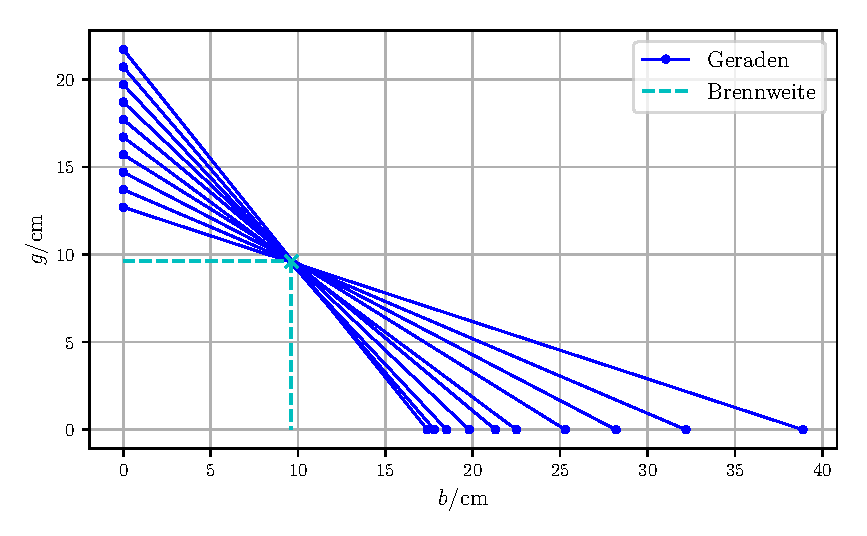
\includegraphics[width=14cm, height=9cm]{build/plot1.pdf}
    \caption{Die Werte für $g$ sind als Schnittpunkte mit der $y$-Achse und die Werte für $b$ sind als Schnittpunkte mit der $x$-Achse dargestellt. Die zueinandergehörenden Werte sind miteinander befunden. Der Schnittpunkt der Geraden ist die gemessene Brennweite.}
    \label{fig:brennweite}
\end{figure}



\subsection{Methode von Bessel}

In Tab. \ref{bessel_weiß} sind die Werte für die Gegenstandsweiten und den Bildweiten bei verschiedenen Abständen von Schirm (Bild) und Gegenstand bei weißem Licht aufgelistet.

\begin{table}\caption{Die ersten Gegenstands- und Bildweiten und die zweiten Gegenstands- und Bildweiten, die mit der Methode von Bessel gemessen wurden, für weißes Licht.}
\label{bessel_weiß}
\centering
\sisetup{round-mode = places, round-precision=1, round-integer-to-decimal=true}
\begin{tabular}{S[]S[]S[]S[]} 
\toprule
{$g_1 / \si{\centi\meter}$} & {$b_1 / \si{\centi\meter}$} & {$g_2 / \si{\centi\meter}$} & {$b_2 / \si{\centi\meter}$}\\
\midrule
12.700000000000003 & 38.0 & 37.400000000000006 & 13.299999999999997\\
12.799999999999997 & 39.900000000000006 & 39.400000000000006 & 13.299999999999997\\
12.400000000000006 & 42.3 & 41.900000000000006 & 12.799999999999997\\
12.200000000000003 & 44.5 & 43.8 & 12.900000000000006\\
12.0 & 46.7 & 46.0 & 12.700000000000003\\
11.900000000000006 & 50.8 & 50.5 & 12.200000000000003\\
11.700000000000003 & 55.0 & 54.5 & 12.200000000000003\\
11.700000000000003 & 57.0 & 56.800000000000004 & 11.899999999999999\\
11.5 & 59.2 & 58.800000000000004 & 11.899999999999999\\
11.400000000000006 & 63.3 & 62.900000000000006 & 11.799999999999997\\
\bottomrule
\end{tabular}\end{table}

\noindent Mit Gleichung \eqref{eqn:e}, Gleichung \eqref{eqn:d} und der Gleichung \eqref{eqn:fbessel} ergibt sich mit den jeweils ersten Werten für die Gegenstands- und Bildweiten für die Brennweite der Linse ein Wert von 
\begin{equation*}
    f_\text{weiß,1} = \SI{9.62 \pm 0.06}{\centi\meter}.
\end{equation*}

\noindent Mit den zweiten Werten ergibt sich für die Brennweite
\begin{equation*}
    f_\text{weiß,2} = \SI{9.89 \pm 0.06}{\centi\meter}.
\end{equation*}

\noindent In Tab. \ref{bessel_rot} sind die gleichen Werte für einen roten Filter und in Tab. \ref{bessel_blau} sind die Werte für einen blauen Filter aufgelistet.

\begin{table}\caption{Die ersten Gegenstands- und Bildweiten und die zweiten Gegenstands- und Bildweiten, die mit der Methode von Bessel gemessen wurden, für rotes Licht.}
\label{bessel_rot}
\centering
\sisetup{round-mode = places, round-precision=1, round-integer-to-decimal=true}
\begin{tabular}{S[]S[]S[]S[]} 
\toprule
{$g_1 / \si{\centi\meter}$} & {$b_1 / \si{\centi\meter}$} & {$g_2 / \si{\centi\meter}$} & {$b_2 / \si{\centi\meter}$}\\
\midrule
13.299999999999997 & 37.400000000000006 & 36.900000000000006 & 13.799999999999997\\
12.900000000000006 & 39.8 & 39.400000000000006 & 13.299999999999997\\
12.5 & 42.2 & 41.900000000000006 & 12.799999999999997\\
12.299999999999997 & 44.400000000000006 & 43.900000000000006 & 12.799999999999997\\
12.200000000000003 & 46.5 & 46.10000000000001 & 12.599999999999994\\
\bottomrule
\end{tabular}\end{table}
\begin{table}\caption{Bessel 2}
\label{bessel_blau}
\centering
\sisetup{round-mode = places, round-precision=1, round-integer-to-decimal=true}
\begin{tabular}{S[]S[]S[]S[]} 
\toprule
{$g_1 / \si{\centi\meter}$} & {$b_1 / \si{\centi\meter}$} & {$g_2 / \si{\centi\meter}$} & {$b_2 / \si{\centi\meter}$}\\
\midrule
13.0 & 37.7 & 37.3 & 13.400000000000006\\
12.799999999999997 & 39.900000000000006 & 39.5 & 13.200000000000003\\
12.600000000000009 & 42.099999999999994 & 41.8 & 12.900000000000006\\
12.299999999999997 & 44.400000000000006 & 44.10000000000001 & 12.599999999999994\\
12.200000000000003 & 46.5 & 46.0 & 12.700000000000003\\
\bottomrule
\end{tabular}\end{table}

\noindent Auf dieselbe Weise wie zuvor ergibt sich, dass die Brennweite für rote Strahlen mit den ersten bzw. zweiten Werten bei 
\begin{align*}
    f_\text{rot,1} &= \SI{9.70 \pm 0.07}{\centi\meter} \\
    f_\text{rot,2} &= \SI{9.92 \pm 0.08}{\centi\meter}
\end{align*}
liegt.

\noindent Für das Licht mit blauem Filter ergeben sich die Brennweiten
\begin{align*}
    f_\text{blau,1} &= \SI{9.67 \pm 0.02}{\centi\meter} \\
    f_\text{blau,2} &= \SI{9.87 \pm 0.05}{\centi\meter}.
\end{align*}



\subsection{Methode von Abbe}
In Tab. \ref{abbe} sind die Gegenstands- und Bildweiten bezüglich des Referenzpunktes $A$ und die jeweilige Bildgröße eingetragen.

\begin{table}\caption{Die Gegenstands- und Bildweiten bezüglich des Referenzpunktes und die jeweiligen Bildgrößen, die mit der Methode von Abbe gemessen wurden.}
\label{abbe}
\centering
\sisetup{round-mode = places, round-precision=1, round-integer-to-decimal=true}
\begin{tabular}{S[]S[]S[]} 
\toprule
{$g' / \si{\centi\meter}$} & {$b' / \si{\centi\meter}$} & {$B / \si{\centi\meter}$}\\
\midrule
27.10000000000001 & 45.599999999999994 & 2.6\\
30.60000000000001 & 44.099999999999994 & 2.3\\
33.900000000000006 & 42.8 & 2.0\\
35.7 & 43.0 & 1.9\\
40.3 & 40.400000000000006 & 1.6\\
42.8 & 39.900000000000006 & 1.5\\
45.7 & 39.0 & 1.4\\
47.3 & 39.400000000000006 & 1.3\\
50.7 & 38.0 & 1.2\\
53.2 & 37.5 & 1.1\\
\bottomrule
\end{tabular}\end{table}

\noindent Die Werte $g'$ sind in Abb. \ref{fig:gstrich} gegen $(1+1/V)$ aufgetragen. In Abb. \ref{fig:bstrich} sind die Werte $b'$ gegen $(1+V)$ aufgetragen.

%Figure gstrich
\begin{figure}
    \centering
    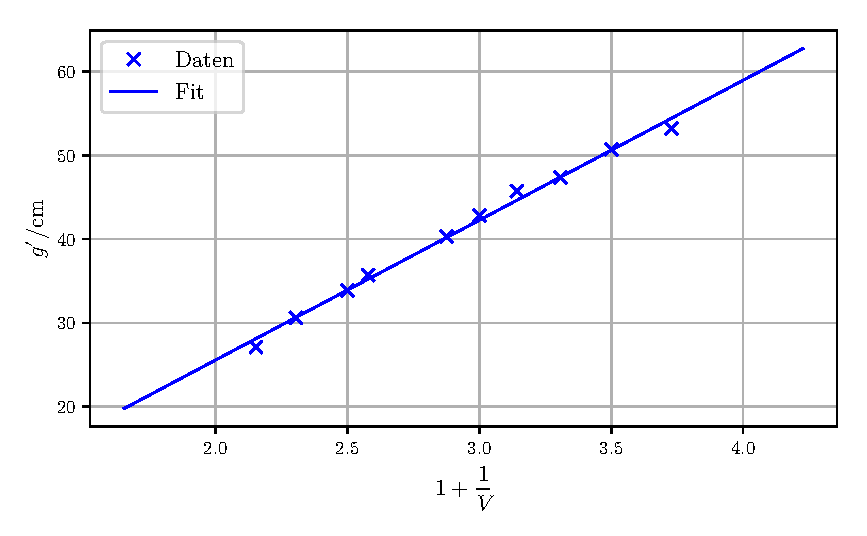
\includegraphics[width=14cm, height=9cm]{build/abbe_g.pdf}
    \caption{}
    \label{fig:gstrich}
\end{figure}

\noindent Die Steigung der Ausgleichsgerade ist nach Gleichung \eqref{eqn:gstrich} die Brennweite.
Der $y$-Achsenabschnitt ist die Entfernung der Hauptebene $H$ zum Referenzpunkt $A$.
Für Abb. \ref{fig:gstrich} ergibt sich die Brennweite zu 
\begin{equation*}
    f_\text{Abbe,1} = \SI{16.69 \pm 0.46}{\centi\meter}
\end{equation*}
und die Hauptebene $H$ des Linsensystems liegt
\begin{equation*}
    h = \SI{-7.82 \pm 1.36}{\centi\meter}
\end{equation*}
entfernt.

%Figure bstrich 
\begin{figure}
    \centering
    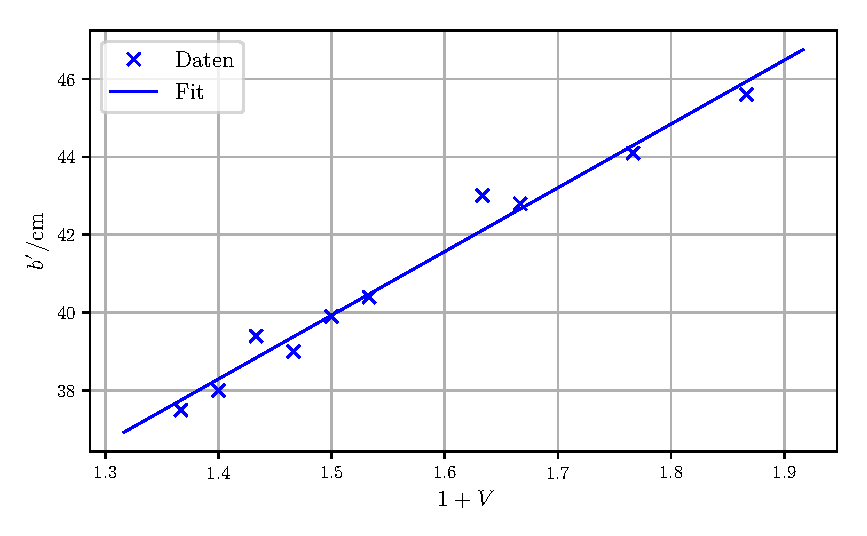
\includegraphics[width=14cm, height=9cm]{build/abbe_b.pdf}
    \caption{}
    \label{fig:bstrich}
\end{figure}

\noindent Analog ist die Steigung der Ausgleichsgeraden in Abb. \ref{fig:bstrich} nach Gleichung \eqref{eqn:bstrich} die Brennweite und der $y$-Achsenabschnitt ist die Entfernung $h'$ der Hauptebene $H'$ zum Referenzpunkt $A$.
Die Brennweite ergibt sich zu 
\begin{equation*}
    f_\text{Abbe,2} = \SI{16.37 \pm 0.89}{\centi\meter}.
\end{equation*}
Die Hauptebene $H'$ des Linsensystems liegt
\begin{equation*}
    h' = \SI{15.37 \pm 1.41}{\centi\meter}
\end{equation*}
entfernt.